% Template LaTeX file for DAFx-08 papers % (fold)
%
% To generate the correct references using BibTeX, run
%     latex, bibtex, latex, latex
% modified...
% - from DAFx-00 to DAFx-02 by Florian Keiler, 2002-07-08
% - from DAFx-02 to DAFx-03 by Gianpaolo Evangelista
% - from DAFx-05 to DAFx-06 by Vincent Verfaille, 2006-02-05
% - from DAFx-06 to DAFx-07 by Vincent Verfaille, 2007-01-05
%                          and Sylvain Marchand, 2007-01-31
% - from DAFx-07 to DAFx-08 by Henri Penttinen, 2007-12-12
%                          and Jyri Pakarinen 2008-01-28
%
% Template with hyper-references (links) active after conversion to pdf
% (with the distiller) or if compiled with pdflatex.
%
% 20060205: added package 'hypcap' to correct hyperlinks to figures and tables
%                      use of \papertitle and \paperauthorA, etc for same title in PDF and Metadata
%
% 1) Please compile using latex or pdflatex.
% 2) If using pdflatex, you need your figures in a file format other than eps! e.g. png or jpg is working
% 3) Please use "paperftitle" and "pdfauthor" definitions below


%%%%%%%%%%%%%%%%%%%%%%%%%%%%%%%%%%%%%%%%%%%%%%%%%%%%%%%%%%%%%%%%%%%%%
%%%%%%%%%%%%%%%%%%%%%%%%%%%%%%%%%%%%%%%%%%%%%%%%%%%%%%%%%%%%%%%%%%%%%
%%%%%%%%%%%%%%%%%%%%%%%%%%%%%%%%%%%%%%%%%%%%%%%%%%%%%%%%%%%%%%%%%%%%%
% 
% TTBlue Notes / Paper
% from conversation with Dave over coffee at Pre en Bulle in Albi
% 20 June 2008
% 
% Allows for:
% * programmatic creation of user interfaces
% * adaptive wrappers for various plug-in architectures (VST, AU, Max/MSP, SuperCollider)
% * dynamic, self-modifying networks of components 
% 
% Dynamic re-configuration of the signal networks and control structures means that TTBlue can be run on a web server and the signal chain defined (or re-defined) in real time on a web client using a GUI (such as a web browser or iPhone) or SMS.
% 
% One application of this is an installation or sculptural art work where you could tweak the behavior by sending it SMS messages using a phone.



%%%%%%%%%%%%%%%%%%%%%%%%%%%%%%%%%%%%%%%%%%%%%%%%%%%%%%%%%%%%%%%%%%%%%
%%%%%%%%%%%%%%%%%%%%%%%%%%%%%%%%%%%%%%%%%%%%%%%%%%%%%%%%%%%%%%%%%%%%%
%%%%%%%%%%%%%%%%%%%%%%%%%%%%%%%%%%%%%%%%%%%%%%%%%%%%%%%%%%%%%%%%%%%%%




%------------------------------------------------------------------------------------------
%  !  !  !  !  !  !  !  !  !  !  !  ! user defined variables  !  !  !  !  !  !  !  !  !  !  !  !  !  !
% Please use these commands to define title and author of the paper:
\def\papertitle{The Jamoma Multicore Audio Graph Layer}
\def\paperauthorA{Timothy Place}
\def\paperauthorB{Trond Lossius}
\def\paperauthorC{Nils Peters}


%------------------------------------------------------------------------------------------
\documentclass[twoside,a4paper]{article}
\usepackage{dafx_08}
\usepackage{amsmath,amssymb,amsfonts,amsthm}
\usepackage{subfigure,color}
\usepackage{euscript}
\usepackage[latin1]{inputenc}
\usepackage[T1]{fontenc}    
%% %%%% for source code listing %%%%%%%%%%%
\usepackage{listings}						% required for source code listings

% Enables multi-line comments:
\usepackage{verbatim} 

\lstset{language=c++}
\lstset{basicstyle=\footnotesize\ttfamily}
\lstset{commentstyle=\color{commentcolor}}
\lstset{tabsize=2}  
\lstset{gobble=2}							% eat the first tab in block listings
\lstset{aboveskip=\bigskipamount}			% amount of space above a block listing
\lstset{belowskip=\bigskipamount}			% ...
%%
\setcounter{page}{1}
\ninept

\usepackage{times}
% Saves a lot of ouptut space in PDF... after conversion with the distiller
% Delete if you cannot get PS fonts working on your system.

% pdf-tex settings: detect automatically if run by latex or pdflatex
%\newif\ifpdf
%\ifx\pdfoutput\relax
%\else
%   \ifcase\pdfoutput
%      \pdffalse
%   \else
%      \pdftrue
%\fi
%\ifpdf % compiling with pdflatex
  \usepackage[pdftex,
    pdftitle={\papertitle},
    pdfauthor={\paperauthorA, \paperauthorB, \paperauthorC},
    colorlinks=false, % links are activated as colror boxes instead of color text
    bookmarksnumbered, % use section numbers with bookmarks
    pdfstartview=XYZ % start with zoom=100% instead of full screen; especially useful if working with a big screen :-)
  ]{hyperref}
  \pdfcompresslevel=9
  \usepackage[pdftex]{graphicx}
  \usepackage[figure,table]{hypcap}
%\else % compiling with latex
%  \usepackage[dvips]{epsfig,graphicx}
%  \usepackage[dvips,
%    colorlinks=false, % no color links
%    bookmarksnumbered, % use section numbers with bookmarks
%    pdfstartview=XYZ % start with zoom=100% instead of full screen
%  ]{hyperref}
%  % hyperrefs are active in the pdf file after conversion
%  \usepackage[figure,table]{hypcap}
%\fi

\title{\papertitle}

%-------------SINGLE-AUTHOR HEADER STARTS (uncomment below if your paper has a single author)-----------------------
%\affiliation{\paperauthorA}    % This command replaces \name{The DAFx Crew}
%{\href{http://www.acoustics.hut.fi/dafx08/}{Dept. of Signal Processing and Acoustics,} \\ Helsinki University of Technology, TKK \\ Espoo, Finland\\
%{\tt \href{mailto:dafx-08@acoustics.hut.fi}{dafx-08@acoustics.hut.fi}}}
%-----------------------------------SINGLE-AUTHOR HEADER ENDS------------------------------------------------------

%---------------TWO-AUTHOR HEADER STARTS (uncomment below if your paper has two authors)-----------------------
%\twoaffiliations{\paperauthorA, \sthanks{This work was supported by the XYZ Foundation}}
%{\href{
%http://www.acoustics.hut.fi/dafx08/}{Dept. of Signal Processing and Acoustics,} \\ Helsinki University of Technology, TKK \\ Espoo, Finland\\
%{\tt \href{mailto:dafx-08@acoustics.hut.fi}{dafx-08@acoustics.hut.fi}}
%}
%{\paperauthorB,\sthanks{This guy is a very good fellow}}
%{\href{http://www.acoustics.hut.fi/dafx08/}{Reading Group, Dept.~of Reading Sciences} \\ Univ.~of Universe, Sun \\ {\tt \href{mailto:dafx-08@acoustics.hut.fi}{dafx-08@acoustics.hut.fi}}
%}
%-------------------------------------TWO-AUTHOR HEADER ENDS------------------------------------------------------

%---------------THREE-AUTHOR HEADER STARTS (uncomment below if your paper has three authors)-----------------------
\threeaffiliations{\paperauthorA}
{\href{http://74objects.com}{74 Objects LLC,} \\ Kansas City, Missouri, USA\\
{\tt \href{mailto:tim@74objects.com}{tim@74objects.com}}
}
{\paperauthorB}
{\href{http://www.bek.no/}{BEK - Bergen Center for Electronic Arts} \\ {\tt \href{mailto:trond.lossius@bek.no}{trond.lossius@bek.no}}
}
{\paperauthorC}%,\sthanks{Is still sore from ice climbing}
{\href{http://www.acoustics.hut.fi/dafx08/}{McGill University} \\ CIRMMT - Centre for Interdisciplinary Research in Music Media and Technology\\McGill University, Montreal, CA\\{\tt \href{mailto:nils.peters@mcgill.ca}{nils.peters@mcgill.ca}}
}
%-------------------------------------THREE-AUTHOR HEADER ENDS------------------------------------------------------

%----------------FOUR-AUTHOR HEADER STARTS (uncomment below if your paper has four authors)-----------------------
%\fouraffiliations{
%\paperauthorA, \sthanks{This work was supported by BEK and GMEA}}
%{\href{http://74objects.com}{74 Objects LLC,} \\ Kansas City, Missouri, USA\\
%{\tt \href{mailto:tim@74objects.com}{tim@74objects.com}}
%}
%{\paperauthorB,\sthanks{This guy is a very good fellow}}
%{\href{http://www.acoustics.hut.fi/dafx08/}{Reading Group, Dept.~of Reading Sciences} \\ Univ.~of Universe, Sun \\ {\tt \href{mailto:dafx-08@acoustics.hut.fi}{dafx-08@acoustics.hut.fi}}
%}
%{\paperauthorC,\sthanks{She is a member of the Wheel Association}}
%{\href{http://www.acoustics.hut.fi/dafx08/}{Spinning Group, Dept.~of Turning Sciences} \\ Univ.~of Planets, Mars \\ {\tt \href{mailto:dafx-08@acoustics.hut.fi}{dafx-08@acoustics.hut.fi}}
%}
%{\paperauthorD,\sthanks{Yes, senior}}
%{\href{http://www.acoustics.hut.fi/dafx08/}{Unknown Group, Dept.~of Volatile Sciences} \\ Univ.~of Nowhere, Somewhere \\ {\tt \href{mailto:dafx-08@acoustics.hut.fi}{dafx-08@acoustics.hut.fi}}
%}
%-------------------------------------FOUR-AUTHOR HEADER ENDS------------------------------------------------------

% (end)

\begin{document}
% more pdf-tex settings:
%\ifpdf % used graphic file format for pdflatex
  \DeclareGraphicsExtensions{.png,.jpg,.pdf}
%\else  % used graphic file format for latex
%  \DeclareGraphicsExtensions{.eps}
%\fi

\maketitle


% TODO: Nils, do you know how to make the footnotes not have the annoying colored boxes around the numbers?
% NP: this is a features from the hyperref package. They don't show up when you print it, so I don't really care about them

%%%%%%%%%%%%%%%%%%%%%%%%%%%%%%%%%%%%%%%%%%%%%%%%%%%%%%%%%%%%%%%%%%%%%%%%%%%%%%%%%%%%%%%%%%%


\begin{abstract}

Jamoma Multicore is a framework for creating graph structures in which unit generators are connected together to process multichannel audio in real-time.  The main applications currently are processing of multichannel audio signals in Max/MSP and PureData as well as live audio coding in Ruby.  Jamoma Multicore forms part of the Jamoma layered architecture.

% particular benefit when dealing with spatial audio
% especially with a massive number of audio channels (Higher Order Ambisonics, WFS, microphone arrays for beamforming)
\end{abstract}


%%%%%%%%%%%%%%%%%%%%%%%%%%%%%%%%%%%%%%%%%%%%%%%%%%%%%%%%%%%%%%%%%%%%%%%%%%%%%%%%%%%%%%%%%%%


\section{Introduction} % (fold)
\label{sec:intro}

Many frameworks, toolkits, and environments for real-time audio processing fuse the issues of creating unit generators with creating graph structures that process audio through those unit generators.  Alternatively, the Jamoma Platform implements a clear separation of concerns, structured in a layered architecture of several frameworks \cite{Place:2010}. Five frameworks currently comprise the Jamoma Platform, providing a comprehensive infrastructure for creating computer music systems. These frameworks are: Jamoma Foundation, Jamoma Graphics, Jamoma Modular, Jamoma DSP, and Jamoma Multicore (see Figure~\ref{fig:layers}). Jamoma Foundation provides low-level support, base classes, and communication systems; Jamoma Graphics provides screen graphics; Jamoma Modular provides a structured approach to development and control of modules in the graphical media environment Max \cite{Place:2006} and Jamoma DSP specializes the Foundation classes to provide a framework for creating a library of unit generators. Jamoma Multicore, the focus of in this paper, is an open source C++ framework providing the ability to create and network Jamoma DSP objects into dynamic graph structures for audio processing\footnote{Licensing is provided under the terms of the GNU LGPL}.  

\begin{figure}[htbp]
\centerline{\framebox{
	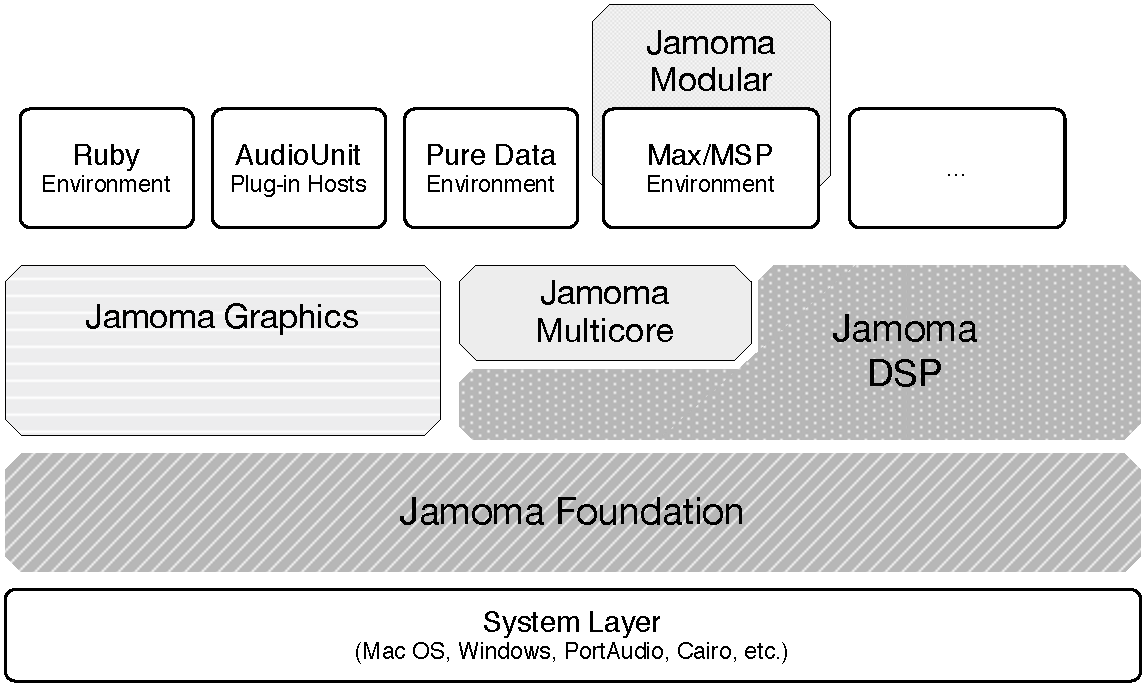
\includegraphics[width=0.9\columnwidth]{../2010-ICMC-DSP/layers-alt}}}
\caption{The Jamoma Platform as Layered Architecture.}
\label{fig:layers}
\end{figure}

% Nils is suggesting that we don't launch in here to say what is different about our stuff, but rather say what we are trying to accomplish [tap]
% Stronger to be able to state what we want -- just a matter of re-phrasing the following.

In addition to the decoupling of the unit generators (Jamoma DSP) from the processing graph, Jamoma Multicore differs from other audio graph architectures in several important ways. %NP: do we need this prev. sentence? isn't that clear ? 
% NP: my suggestion: we should do this section similar to the intro of the DSP paper 1. state our requirements 2. background review 3. explain our solution
 First, the connections between objects in the graphs are multi-channel connections; any given connection may carry N channels of audio.  Second, the content carried by the connections is dynamic; the number of channels, the size of the sample vectors, and the sample-rate of the audio can change during runtime operation.  Third, the type of graph used relies on a \emph{pull} pattern which is readily adapted to multi-threaded parallel calculations.

An additional design difference between Jamoma Multicore and most other audio processing graph software is the use of a peer object model.  The peer object model abstracts the implementation and execution of the graph from any particular environment or platform.  This allows for implementations of Jamoma Multicore to be readily implemented for any number of environments.  To date the authors have created implementations for Max, PureData, Audio Units, and Ruby.
% NP: the term peer object model is unclear to me -- maybe the whole peer-object thing should go into the background

% TODO For list of requirements:  Decoupling Graph and Unit Generator

%- presenting distinguishing between graph and units
%    - what is a graph and a unit?
%
%- requirements?
%    - be able to construct graphs
%    - multichannel as configurable 
%    - live coding (or introspection blah blah)
%  
%- additional niceties:
%    - environment-agnostic (cross-coding -  ability to prototype and wrap as plug-ins)
%
%- application for Jamoma Multicore
%    - e.g. up/downmixing; encoding/decoding 

% (end)



%%%%%%%%%%%%%%%%%%%%%%%%%%%%%%%%%%%%%%%%%%%%%%%%%%%%%%%%%%%%%%%%%%%%%%%%%%%%%%%%%%%%%%%%%%%

\section{Background} % (fold)

% TODO: _really_ stress multichannel throughout

% TODO: begin with the historical background -- the difficulty of patching multichannel/ambisonic object networks in MSP, etc. etc. etc.

\subsection{Audio Graph Structures} % (fold)

A graph structure is an abstract structure where paths are created between nodes. %NP: what is a node?
 The paths between these nodes then define the data-flow of the graph.  Graphs targeting audio processing employ several patterns and idioms to achieve a balance of efficiency, flexibility, and real-time capability.

Environments for processing typically need to address concerns in both synchronous and asynchronous contexts.  Asynchronous communication is required, for example, by MIDI and for driving attributes from DAW automation.  Conversely, realtime processing of audio streams must be handled synchronously.  Most environments, such as CLAM  \cite{Amatraian:2007}, deal with these two types of graphs as separate from each other.  In the Jamoma Platform this is also the case, where Jamoma Multicore comprises the synchronous audio graph concerns.
% TODO: Is the synchronous/asynchronous a tad to specific here and we are rather thinking in terms of audio rate and control rate? In Csound e.g. we are talking k-rate and a-rate. k-rate is processed at a lower sample rate than a-rate, but to the best of my knowledge is still synced to the audio processing. - TL

% TODO: The following paragraph seems like it is really starting to veer off into implementation and not just background -- tap
% TODO: maybe we can just cut the block processing part entirely -- does it _really_ matter for the purposes of section 3? -- tap

These synchronous calls encourage or enforce the notion of \emph{frame processing}.  Jamoma Multicore processes blocks of samples at once rather than a single sample at a time.  These blocks of samples are passed using the Jamoma DSP class for audio signals, which bundles vectors of audio for multiple channels together with an interface for accessing the signal data and metadata.

% This might be conflicting with how Gabor is able to work on vectors of dynamically changing size, e.g. for Yin analysis or whatever it is called...

% (end)


\subsection{Push vs. Pull} % (fold)

When visualizing a graph for DSP processing, it is common to represent the flow of audio from top to bottom or left to right.  Under the hood, the processing is often implemented in this top-to-bottom flow as well.  Audio at the top of the graph `pushes' down through each subsequent object in the chain until it reaches the bottom.

Alternatively, audio processing may be driven from the bottom of the chain from a `terminal object' or `sink'.  This `pull' method for processing and audio graph is used by several environment's including Apple's AUGraph and ChucK \cite{wang:2008}.  AUGraph and ChucK are subject to certain limitations however: AUGraph does not permit ``fanning'' connections (many inlets connected to one outlet and vice-versa) while ChucK is not multithreaded.

% TODO: do we need to cite a source or add a footnote for the AUGraph documentation about this fanning thing?

% (end)


\subsection{Multichannel Processing} % (fold)

In many patching environments for real-time audio processing, such as Max, Pd, Bidule and AudioMulch, audio objects are connected using mono signals. For multichannel spatial processing the patch has to be tailored to the number of sources and speakers. If such programs are considered programming environments and the patch the program, a change in the number of sources or speakers requires a rewrite of the program, not just a change to one or more configuration parameters.

% TODO: do we need citations for Max, Pd, Bidule, and AudioMulch?

% Here's a resource on spatialisation in Pd:
% http://grh.mur.at/misc/PdSpatialization.tar.gz

In Csound multichannel audio graphing is extended somewhat through the introduction of the Zak Patch System, enabling flexible patching or routing from one instrument to another. One advantage of the Zak system over global variables is that communication between instruments may be reconfigured in the score without requiring changes to the orchestra \cite{Mikelson:2000}. One example is the \texttt{vbapz} opcode for multichannel vector-base amplitude panning, using a ZAK array for output.

% TODO: In the above paragraph we are introducing a new concept: global variables -- where does this come from, and what does it have to do with anything?

\begin{comment}

From the Csound Manual:

The zak opcodes are used to create a system for i-rate, k-rate or a-rate patching. The zak system can be thought of as a global array of variables. These opcodes are useful for performing flexible patching or routing from one instrument to another. The system is similar to a patching matrix on a mixing console or to a modulation matrix on a synthesizer. It is also useful whenever an array of variables is required. 

The zak system is initialized by the zakinit opcode, which is usually placed just after the other global initializations: sr, kr, ksmps, nchnls. The zakinit opcode defines two areas of memory, one area for i- and k-rate patching, and the other area for a-rate patching. The zakinit opcode may only be called once. Once the zak space is initialized, other zak opcodes can be used to read from, and write to the zak memory space, as well as perform various other tasks. 

Zak channels count from 0, so if you define 1 channel, the only valid channel is channel 0. 

\end{comment} 


By comparison, SuperCollider has an elegant way of representing multiple channels of audio as arrays. When an array of audio signals is given as input to a unit generator it causes multichannel expansion: multiple copies of the unit generator create an array of unit generators, each processing a different signal from the array of inputs. In the following example a stereo signal containing white and pink noise is filtered:

\begin{lstlisting}
\ {
		\\ Create stereo signal as array:
		p = [WhiteNoise.ar, PinkNoise.ar];
		
		\\ Biquad filter applied to array of channels:
		SOS.ar(p, 1, -1.992, 0.986, 1.992, -0.993, 0.1);
\ }.play
\end{lstlisting}

% TODO: Below is an excerpt from the Csound multichannel example provided by �yvind Brandsegg:
% TODO: Change tabs to spaces for better text rendering in paper

\begin{lstlisting}
**************************************************
; multichannel filter, event handler
	instr 2
	iNumC	= p4	; number of channels
	iCF		= p5		; filter cutoff
	ichnNum	= 0		; init the channel number
makeEvent:
	ichnNum	= ichnNum + 1
	event_i	"i", 3, 0, p3, ichnNum, iCF
	if ichnNum < iNumC igoto makeEvent
	endin

; multichannel filter, audio processing
	instr 3	
	instance	= p4
	iCF			= p5
	Sname		sprintf	"Signal_%i", instance		
	a1			chnget	Sname
	a1			butterlp a1, iCF
				chnset	a1, Sname
	endin
;***************************************************
\end{lstlisting}  


\begin{comment} % (fold)
NP: my research into multichannel capabilities with SC\\
seems to be simple\\     
a) making a 3 channel  Sine Oscillator 

\begin{lstlisting}
{ Out.ar( 0, [ SinOsc.ar, SinOsc.ar, SinOsc.ar ] ) }.play;
\end{lstlisting}
b) making a 24 channel sine wave oscillator in SC:
\begin{lstlisting}
{ Out.ar( 0, SinOsc.ar.dup(24) ) }.play;
\end{lstlisting}  

for more complex multichannel handling by a system called Multichannel Expansion, see \url{http://danielnouri.org/docs/SuperColliderHelp/Other%20Topics/MultiChannel.html}
\end{comment} 
% (end)

% Trond investigationg SuperCollider:

\begin{comment}

% Example 1: Read stereo sound file, apply filter to both channels, and output:

(
b = Buffer.read(s, "/Users/lossius/Music/AIFF/VT Mandela_lyd/Lange/klokkerhav.aif");

{ 	var sig, rho, theta, b1, b2;

	theta = MouseX.kr(0.2pi, pi);
	rho = MouseY.kr(0.6, 0.99);
	b1 = 2.0 * rho * cos(theta);
	b2 = rho.squared.neg;

	sig = PlayBuf.ar(2, b, BufRateScale.kr(b), doneAction:2);
	
	// This is elegant, both channels are filtered with same coefficients:
	SOS.ar(sig, 1.0, 0.0, 0.0, b1, b2)

}.play
)


% Example 2: Pink noise => ambisonic encoding => encoded signal is filtered => ambisonic decoding => out

% ******************************************
% Ambisonics: 1 source, 4 speakers
% ******************************************

(
{
	var ambi, a, rho, theta, b1, b2;
	
	// Mouse stuff controlling filter
	theta = MouseX.kr(0.2pi, pi);
	rho = MouseY.kr(0.6, 0.99);
	b1 = 2.0 * rho * cos(theta);
	b2 = rho.squared.neg;
	
	// sources
	p = PinkNoise.ar;
	
	// B-format encode
	ambi = PanB2.ar(p, MouseX.kr(-1,1), 0.1); 

	// Now we do some weird filtering, with same coefficients for each of the encoded channels:
	ambi = SOS.ar(ambi, 1.0, 0.0, 0.0, b1, b2);
	
	// B-format decode to quad
	a = DecodeB2.ar(4, ambi[0], ambi[1], ambi[2]);
	
	// reorder to my speaker arrangement: Lf Rf Lr Rr
	a.at([0,1,3,2])
}.play;
)


% ******************************************
% Ambisonics: 2 source, 4 speakers
% ******************************************

(
{
	var ambi, a;
	
	// sources
	p = [PinkNoise.ar, WhiteNoise.ar];
	
	// Now we do peak notch filtering. Coefficients from Max, but b1 and b2 have their signs swapped in SuperCollider
	// 1.006468 -1.992072 0.986487 -1.992072 0.992955
	// 1.030371 -1.932701 0.928888 -1.932701 0.959259
	p = SOS.ar(p, [1.006468, 1.030371], [-1.992072, -1.932701], [0.986487, 0.928888], [1.992072, 1.932701], [-0.992955, -0.959259], 0.1);
	
	// B-format encode
	ambi = PanB2.ar(p, [MouseX.kr(-1,1), 1-MouseX.kr(-1,1)], [0.6, 0.1]); 
	
	// B-format decode to quad
	a = DecodeB2.ar(4, ambi[0][0]+ambi[1][0], ambi[0][1]+ambi[1][1], ambi[0][2]+ambi[1][2]);
	
	// reorder to my speaker arrangement: Lf Rf Lr Rr
	//a.at([0,1,3,2])
}.play;
)


\end {comment} 
% (end)

% Investigate ChucK:

\begin{comment}

Examples of arrays here, although I'm not sure yet if this at all relates to audio multichannel signals:
http://chuck.cs.princeton.edu/doc/examples/

Multichannel example:
https://ccrma.stanford.edu/~jchrsmt/Compose/Chuck/enginedrone.ck

Jeff Smith (2007) toolkit for building multi-channel sound in chuck. Examples included:
https://ccrma.stanford.edu/~jchrsmt/Compose/Chuck/nchannel4.ck
https://ccrma.stanford.edu/~jchrsmt/Compose/Chuck/nchannel8.ck
https://ccrma.stanford.edu/~jchrsmt/Compose/Chuck/nchannel16.ck
https://ccrma.stanford.edu/~jchrsmt/Compose/Chuck/nchannel18.ck

\end{comment} 


% TODO: Who else has a true multichannel environment?  anyone?

% (end)


\subsection{Decoupling Graph and Unit Generator} % (fold)

Jamoma DSP does not define the way in which one must produce signal processing topographies.  Instead, the process of creating objects and connecting them are envisioned and implemented orthogonally and the graph is created using a separate framework known as Jamoma Multicore.  Thanks to this decoupling of Jamoma DSP and Jamoma Multicore we are able to create and use Jamoma DSP unit generators with a number of different graph structures.  Jamoma Multicore is one graph structure that a developer may choose to use\footnote{However unlikely, it is also theoretically possible to use Jamoma Multicore with an alternative unit generator library}.

Max, Pd, SuperCollider, Csound, Bidule, AudioMulch, Reaktor, Reason all have have units, but the units can only be used within the particular environment. The units have a proprietary format for unit generators, so there's no interchangeability, and likewise the graph structure is proprietary. While SDKs are available for some of them, for others no SDK exists at all and they are proprietary. Ability to host Audio Units and VST extends these environments, but with limitations.

% TODO: Also mention flext, enabling shared code between Max and Pd. Does it still work with Max 5? - TL
% 			I don't think flext is worth mentioning - TAP

% (end)

% (end)

%%%%%%%%%%%%%%%%%%%%%%%%%%%%%%%%%%%%%%%%%%%%%%%%%%%%%%%%%%%%%%%%%%%%%%%%%%%%%%%%%%%%%%%%%%%


\section{Design and Implementation} % (fold)

\subsection{Structure} % (fold)

Jamoma Multicore is a framework \footnote{We use the term framework in a generic sense, as a dynamically linked library together with supporting source and an API.} implementing a synchronous multichannel audio processing graph driven using a pull methodology.  This is accomplished through the creation of a node class for the graph, \texttt{TTMulticoreObject}, which wraps a unit generator with other supporting objects.  \texttt{TTMulticoreObject} then manages these instances and the information necessary to pull samples from its sources.

% TODO: in the figure we should label the white box with the rounded corners as TTMulticoreObject -- TAP

\begin{figure}[htbp]
\centerline{\framebox{
	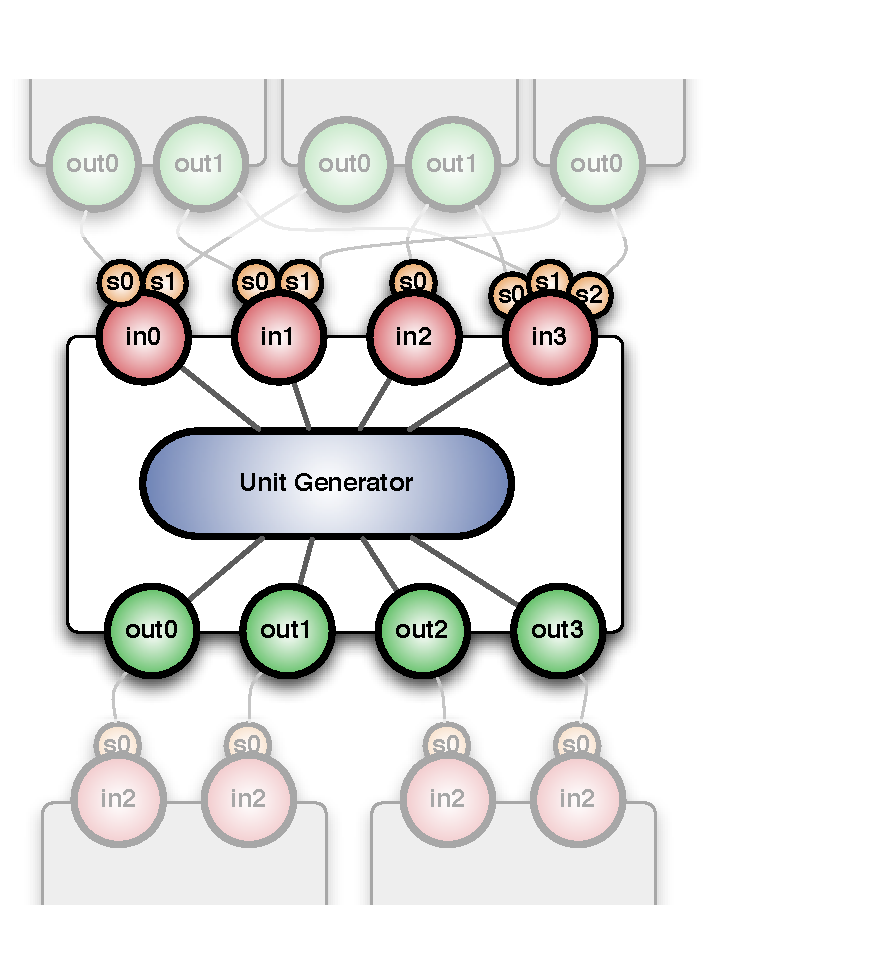
\includegraphics[width=0.9\columnwidth]{anatomy-compact}}}
\caption{MulticoreObject Class Anatomy}
\label{fig:anatomy}
\end{figure}

Figure \ref{fig:anatomy} shows these classes and how they are related. In the figure an object is connected to three upstream objects, and to two downstream objects, with all connections being multichannel.  A connection between objects can be considered to be a many-to-many association; each outlet can be connected to many inlets, and each inlet can be connected to many outlets. The source objects represented by $s0$, $s1$, etc. can then be considered as join tables representing each connection in the many-to-many relationship individually.

The architecture of \texttt{TTMulticoreObject} is layered: the Multicore object itself only knows about its inlets; the inlets only know about their sources (joins); the sources know about what object and from which outlet they are connected. In the figure this is illustrated by the object having four inlets. Two multichannel sources $s0$ and $s1$ are connected to the first inlet $in0$, two to the second, and so on. In short:

				A graph has many objects.\\
\indent	An object has many inlets.\\
\indent	An inlet has many sources.\\
\indent	A source has many channels.\\

% From Rails book:
% Within the database, many-to-many associations are implemented using an intermediate join table. This contains foreign key pairs linking the two target tables. Active Record assumes that this join table’s name is the concatenation of the two target table names in alphabetical order. In our example, we joined the table categories to the table products, so Active Record will look for a join table named categories_products.

% (end)


\subsection{Building the Graph} % (fold)

For processing to occur, the connections of the graph must be established and the graph readied for operation.  This is done by first passing a source object and the outlet and inlet number of the connection to the downstream object's \texttt{connect()} method.  Similarly, connections may be cut by passing the same information to the downstream object's \texttt{drop()} method.  Connections may be created or cut at any time before, after, or during the graph being processed.  There is no global signal chain compilation; the graph may dynamically change over the course of a performance.

% (end)


\subsection{Processing the Graph} % (fold)

All processing is driven by the object at the end of the processing chain according to a two step process.  First, a `preprocess' method is propagated up the chain from the terminal object.  This zeroes buffers and sets flags that indicate each object's processing state.  It is of no consequence if an object receives multiple preprocess calls, such as would happen if there are multiple terminal nodes.

Since Jamoma Multicore is using a pull-based architecture, an object's \emph{outlets} are passive.  They are simply buffers storing the output calculated by the wrapped unit generator.  The unit generator is simply an instance of a Jamoma DSP class, specified as an argument when the \texttt{TTMulticoreObject} is instantiated.  This unit generator is responsible for actually calculating the audio to be stored by the outlet buffers.

Unlike the outlets, the \emph{inlets} are active.  When asked for a vector of audio by the unit generator, they then each request audio from all of their sources (other objects' outlets).  If an inlet has multiple sources, those sources are summed.  When all of the inlets have performed this operation, then the unit generator proceeds to process the audio buffered in the inlets and fills the buffers in the outlets.  Sources manage a one-to-one connection between an inlet and an outlet; inlets may have zero or more sources.  To summarize:

With the objects in the graph prepared by the \texttt{preprocess()} call, the audio can be pulled from the graph by a terminal object using the \texttt{process()} call on each of its sources.

% TODO: We need to discuss what we do in the case that one inlet have several sources with differing numbers of channels 

% Third, we could send a post-process message, but we don't at the moment.
% But what would the purpose of it be? What would this be able to do that could not just as easily be done as part of the next "preprocess" step? The only thing I can imagine currently that this would be useful for, would be to schedule asynchronous events. On second thought that might actually be useful, e.g. for updating GUI objects showing signal levels etc., or for banging control-rate events based on monitoring and analyis of audio signals... [TL]

% (end)


\subsection{Graph Description} % (fold)

Given a Jamoma Multicore graph, the topology can also be traversed for purposes other than directly calculating audio.  
Any node in a Jamoma Multicore graph can be queried to create a description.  The returned \texttt{TTMulticoreDescription} object will then provide 
metadata about the entire graph as seen through that object's inlets.  
There are many applications of this description, including visual representation of the graph, statistical analysis, and cross-coding.

% (end)


% (end)



%%%%%%%%%%%%%%%%%%%%%%%%%%%%%%%%%%%%%%%%%%%%%%%%%%%%%%%%%%%%%%%%%%%%%%%%%%%%%%%%%%%%%%%%%%%

\section{Application} % (fold)

\subsection{Max/MSP} % (fold)

Show it working in Max/MSP
% TODO: need a screenshot demonstrating multi-channel


\begin{figure}[htbp]
\centerline{\framebox{
	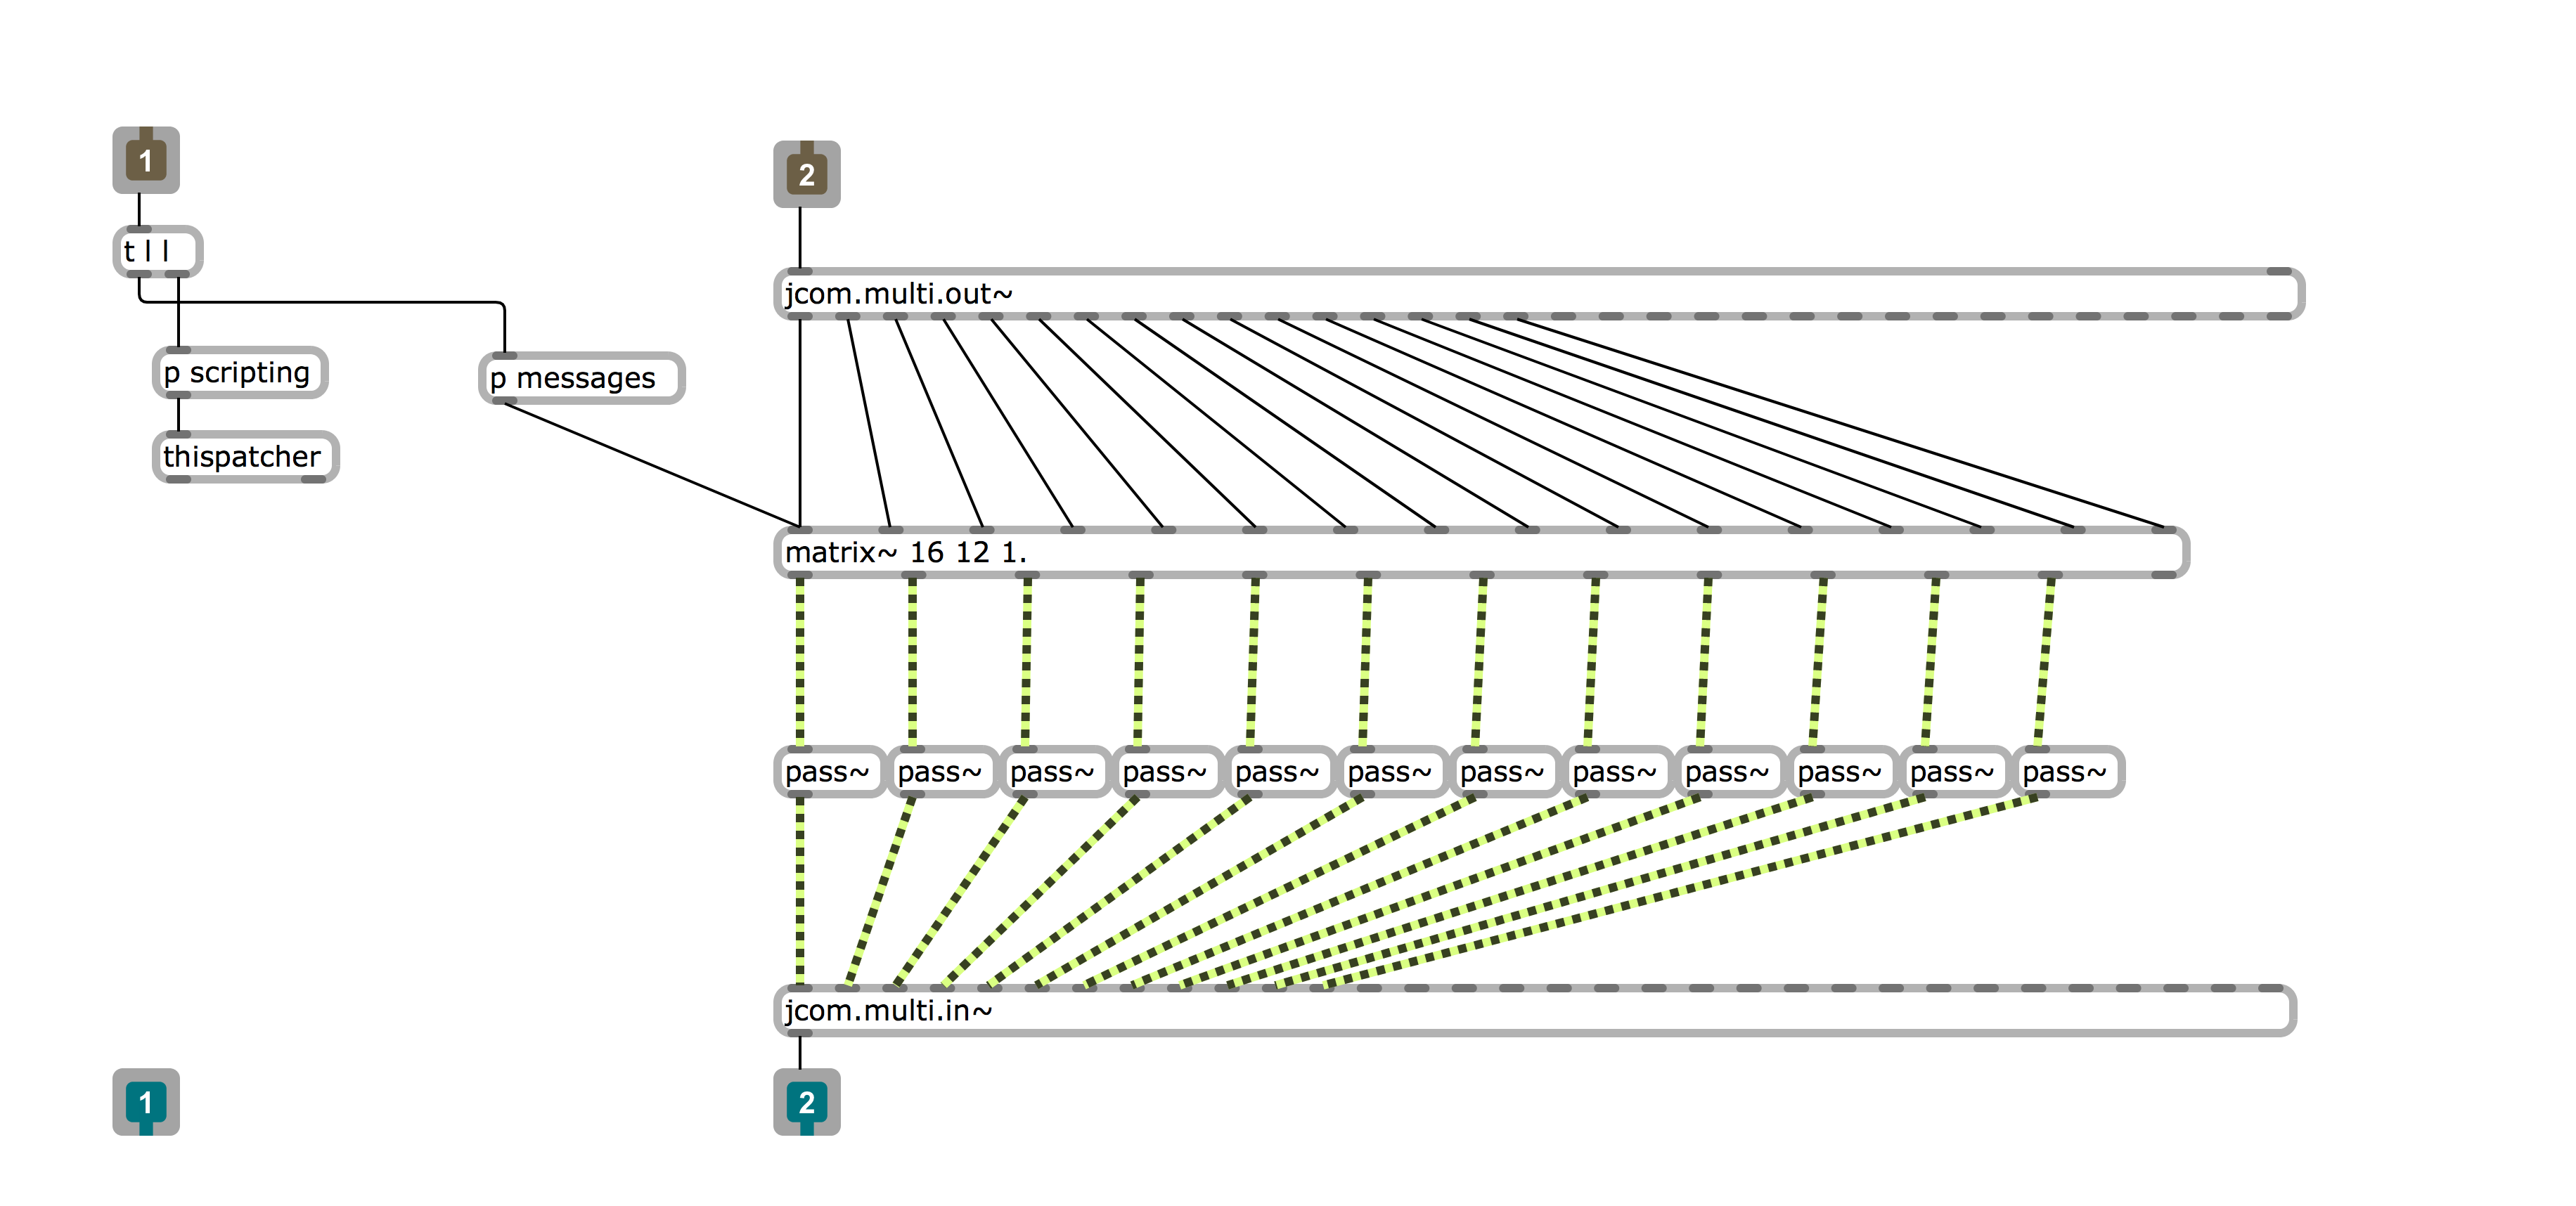
\includegraphics[width=0.9\columnwidth]{jalg-sur-vbap-sans-multicore}}}
\caption{Max patcher without multicore}
\label{fig:max-after}
\end{figure}


\begin{figure}[htbp]
\centerline{\framebox{
	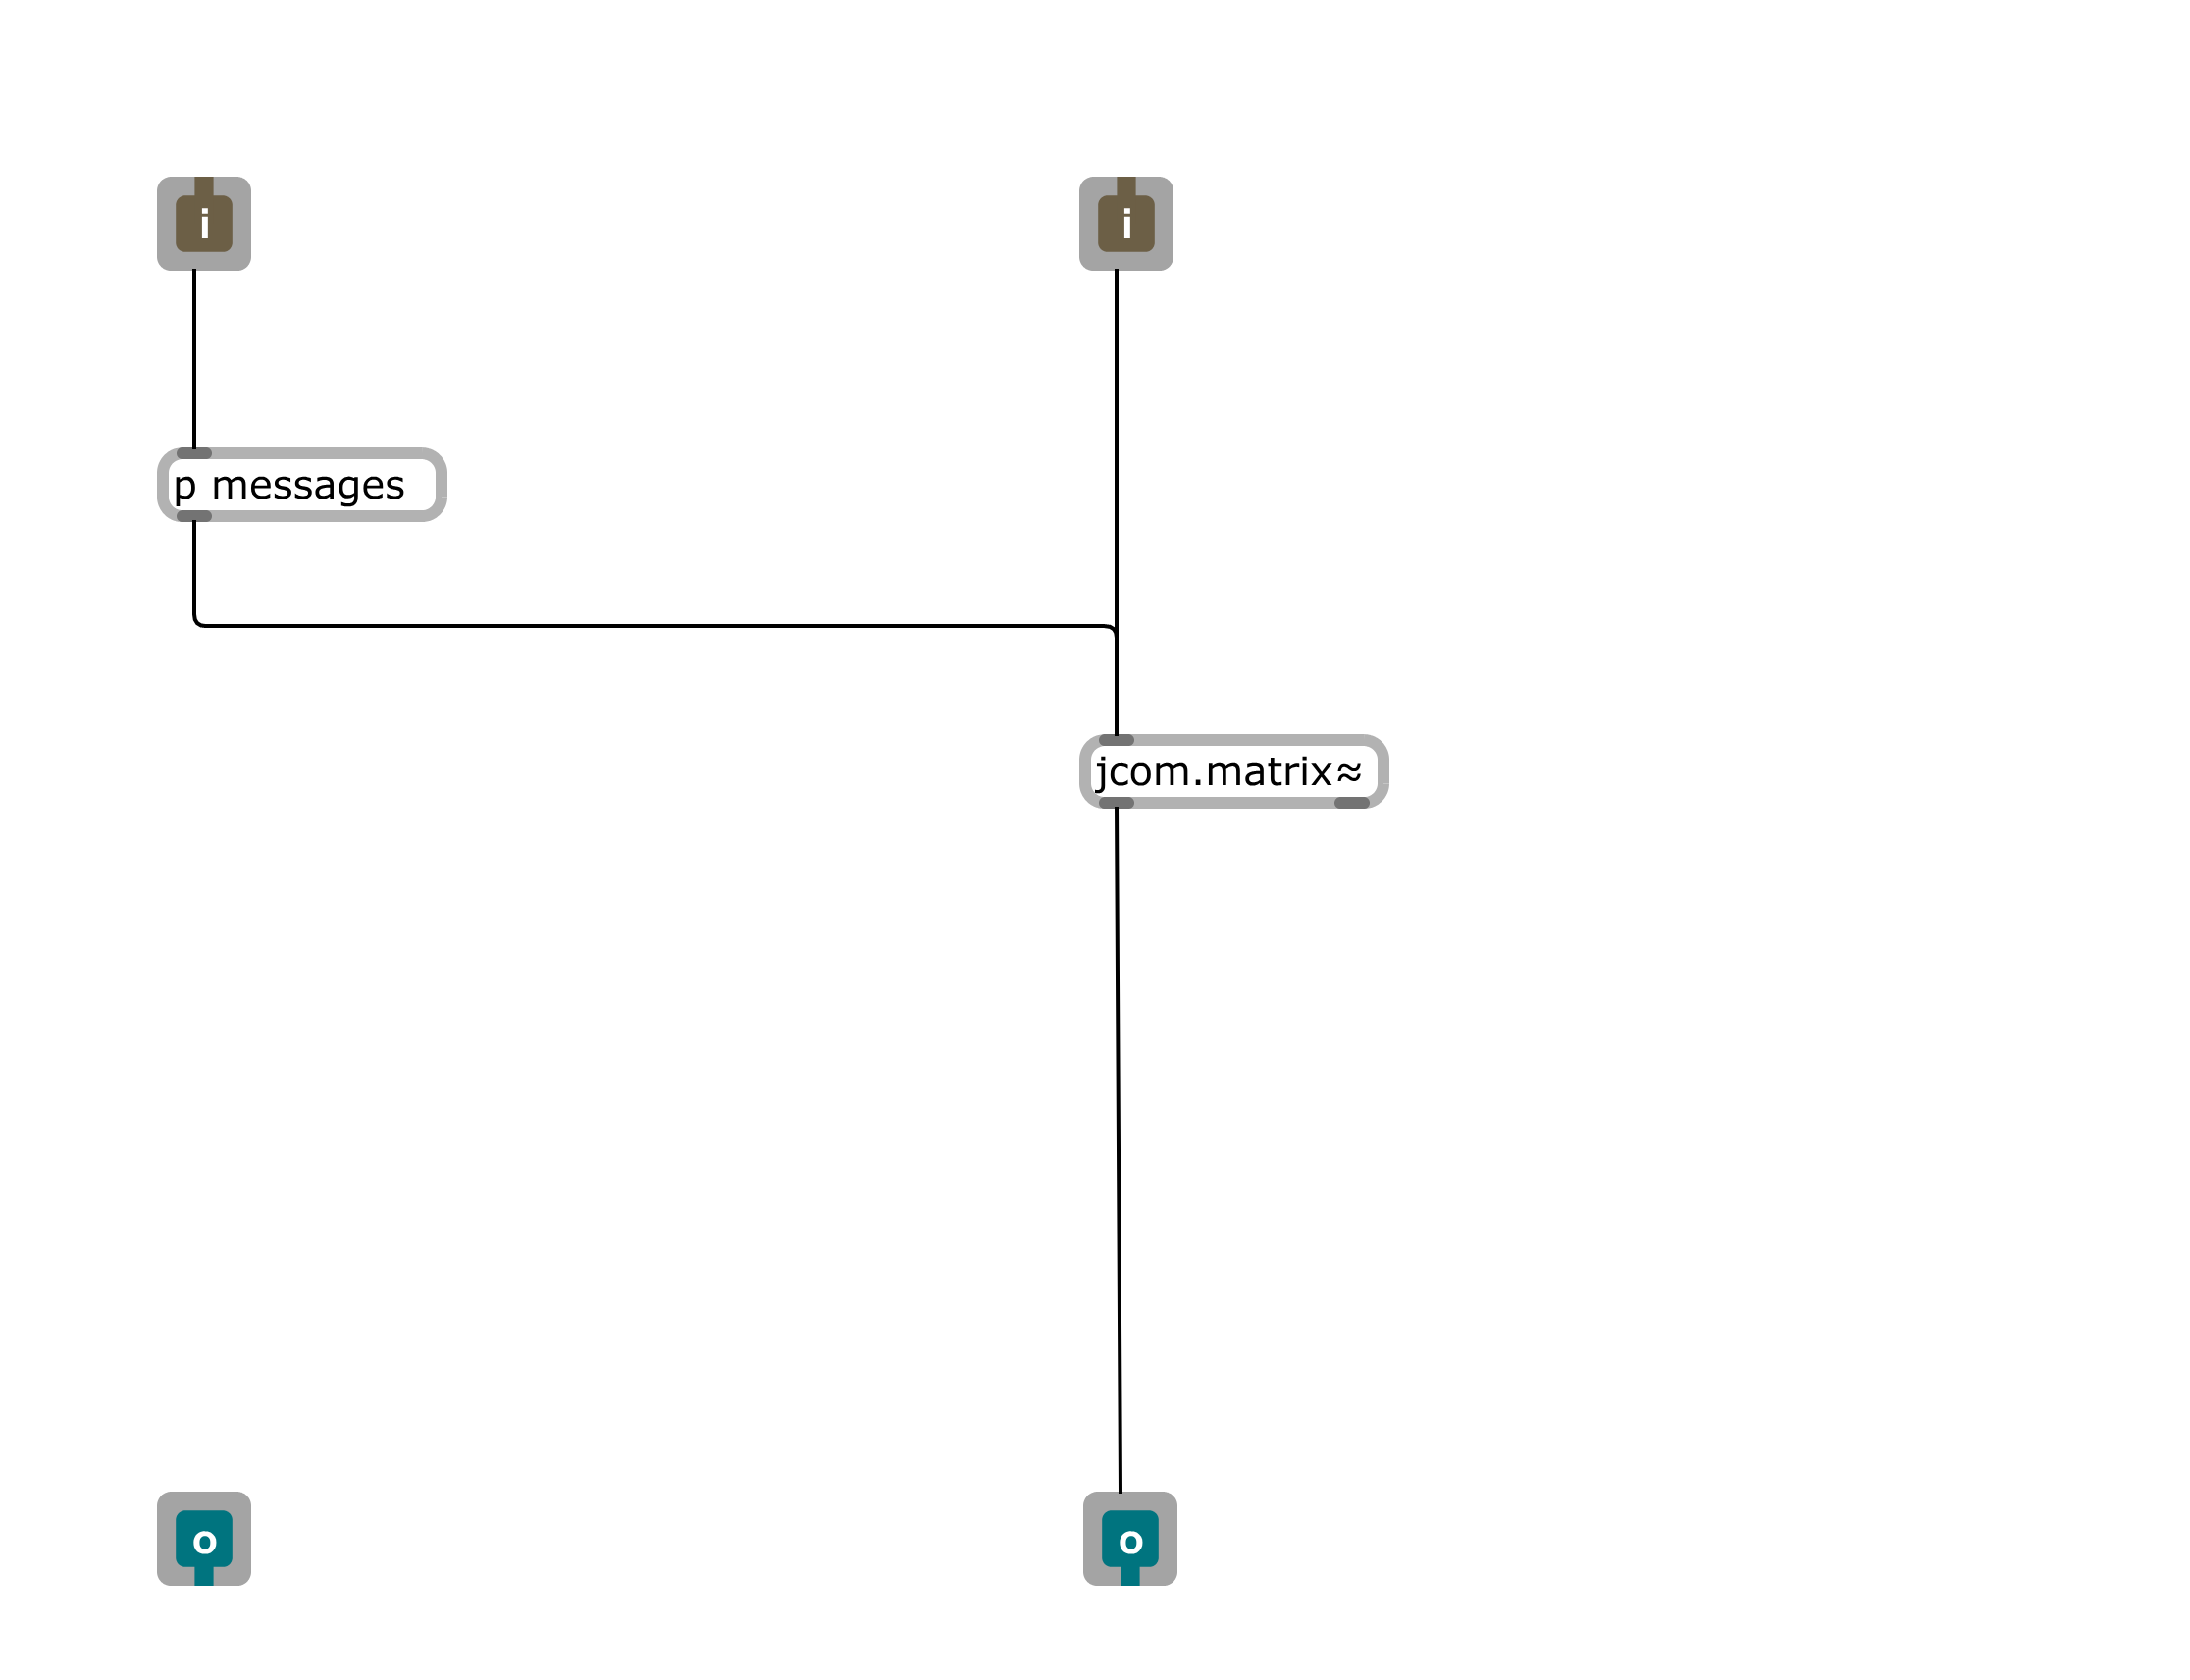
\includegraphics[width=0.9\columnwidth]{jalg-sur-vbap-avec-multicore}}}
\caption{Max patcher with Multicore}
\label{fig:max-before}
\end{figure}


\subsubsection{Jamoma Modular} % (fold)

Nils Says:
There is a new modular branch to start working with the multicore 
externals. The name of the branch is ``0.6-multicore''.

So far, I mainly introduced in= and out= in a couple of modules. more to come.
jmod.sur.multi.in
jmod.sur.multi.out
jmod.sur.multi.input
jmod.sur.multi.aux
jmod.sur.meters
jmod.sur.output
jmod.sur.vbap
jmod.sur.dbap

% TODO: these last two require a matrix that operates on the channels within a signal, not on multiple signals

So you can start to connect your modules and see what's working and 
what's not.
If you are curious, just check out this branch and try it.
in the git repository, go to Modules/Modular and do a

git checkout 0.6-multicore

% Some important things to keep in mind:
% - Priorities, how to we control the order of operations?    We don't at the moment (which is like Pd, but unlike Max)
% - Matrix mixer/router development, with particular thought about what happens when 5.1 audio is routed to stereo etc.
% - Signals of varying data rate (for example as proposed by Pulkki), e.g. compressed signals or higher res signals
% - Signals of steady data rate but varying vector/buffer size (as in FTM/Gabor)

Dynamic number of channels (perhaps useful for FFT and spectral processing?)

% Would be ideal if we could have a wrapper for standard MSP external objects as Multicore objects. 
% Call the DSP method directly from this wrapper?
% Create our own internal DSP chain for it?
% start simple as with biquad~, meaning 1 in and 1 out...
% it seems like the easiest way out is to just use patcher scripting.


% (end)

One difference to Max/MSP and Pd is that the signal network can be reconfigured dynamically without requiring a 'recompile' of the signal chain.  This is addressed through Jamoma Multicore -- Jamoma DSP is low level and is agnostic about how objects are combined into a network or topology.

However, objects can be recombined and structured at runtime, offering the same kind of flexibility and "expressive power".

% (end)


\subsection{PureData} % (fold)

Similar to the implementation of Jamoma Multicore for Max, there is also a Jamoma Multicore implementation for Pd. Figure \ref{fig:pd} demonstrates the use of Jamoma Multicore in Pd for passing 4 channels through a chain for processing, taking advantage of the multichannel patch cord connections.

\begin{figure}[htbp]
\centerline{\framebox{
	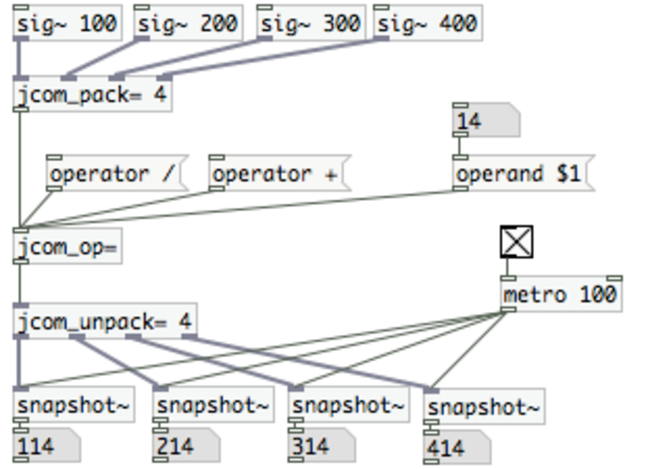
\includegraphics[width=0.9\columnwidth]{multicore-pd}}}
\caption{Simple Pd document processing 4 channels with Jamoma Multicore}
\label{fig:pd}
\end{figure}

% (end)


\subsection{Ruby} % (fold)

As mentioned, Jamoma Multicore is ideally suited for use in many different environments. This includes not only graphical environments, but textual environments as well.  The authors have created an implementation of Jamoma Multicore for the Ruby language environment.  Ruby is offers a wealth of application areas include web development using Ruby On Rails\footnote{http://rubyonrails.org} and Live Coding\cite{Collins:2003} using \emph{irb}.  The following listing demonstrates a simple \emph{irb} session:

\begin{lstlisting}
  require 'TTRuby'
  dac = TTAudio.new "multicore.output"
  osc = TTAudio.new "wavetable"
  dac.connect osc
  dac.send "start"
  osc.set "frequency", 220.0
\end{lstlisting}

By using Jamoma Multicore in the Ruby environment for Live Coding users are able to access all of the benefits of using a popular, general purpose language while at the same time gaining access to many of the benefits of a domain specific language for musical performance such as ChucK

% TODO: Are there any published articles specifically about using irb for live coding performance?

% (end)


\subsection{Cross-Coding} %(fold)

Using the capabilities of a graph to produce a description of itself, we are able port code across environments in a variety of formats.  For example, we have implemented functions that export a graph created in Max to a Ruby source file.  Likewise we can export from a Ruby source file to Pd and from a Pd canvas to C++ code.  

The ability to export code/patcher/canvas/document from any supported environment to any other supported environment offers great flexibility, not only for code generation and prototyping, but for freedom in sharing work across platforms and with colleagues.  The currently supported export formats are: Max 5 patcher, C++ source code, Ruby source code, PureData.

% (end)


% (end)


%%%%%%%%%%%%%%%%%%%%%%%%%%%%%%%%%%%%%%%%%%%%%%%%%%%%%%%%%%%%%%%%%%%%%%%%%%%%%%%%%%%%%%%%%%%

\section{Discussion and Future Work} % (fold)

% TODO: we need an object like out≈ that drives a graph outside of real time to fill a buffer~ or jit.matrix
% TODO: trond or nils -- do you have some interesting applications of the above?
% TODO: If we are presenting a graph system, should we discuss the potential (if any) for expanding this from being a graph system for audio processing, to video processing or other kinds of time-tagged data, along the line of e.g. Max/Jitter, QuartzComposer or Octane?
% TODO: Discuss the potential for work on spatialisation, and further work in this direction...
% TODO: Non-PCM streams?  The need for audio signal metadata?
% TODO: Also talk about the Jamoma Graph thing?


\subsection{Multiple Simultaneous Graphs} % (fold)

By it's nature, a Multicore graph is defined as all objects connected together into a graph structure terminating at a terminal object that drives the graph.  There is no limitation on how many of these graphs may exist independently, and simultaneously, in any environment.  As these graphs are fully-independent of each other they may run at different rates, in different threads, and addressing different hardware.  The independent graphs may even run side-by-side with one running in real-time while another is operating out of real time.

% (end)


\subsection{Multithreading} % (fold)

The structure of Jamoma Multicore is ideal for distributing processing of the graph amongst parallel threads.  Currently it is already possible run separate graphs on separate threads.  More powerful and dynamic opportunities arise when a graph itself is distributed to parallel threads.  

The authors are continuing to explore ways by which integrated analysis and benchmarking can be made a part of nodes on the graph.  The data generated by this instrumentation can then drive thread-spawning decisions in real-time, particularly where bifurcations of the graph are present.  We hope that this intelligent and adaptive multithreading will be able to maximize performance on multi-processor hardware.

%    - multithreading where applicable
%    - pragmatic multithreading: real-time statistics for optimizing between different processors
%   
%A   B
% \ /
%  C


% TODO: Grand Central Dispatch (GCD) is now open source, is this relevant?

% TANGA provides and interesting environment because the audio engine is explicitly multi-threaded and thus multi-core capable\cite{Reiter:2007}.  However, it doesn't fit the bill because it is targeted at one context: MPEG-4 scene rendering.  We need something more general.  And it doesn't matter because we are thread-agnostic.

% (end)


% TODO: Is there any other environment that we should acknowledge?


% Multithreading is a big deal \cite{asanovic2008parallel}, \cite{multicoreICMC08}.  We can easily operate multiple graphs in their own threads as previously mentioned.  However, there are many opportunities for parallel processing within a single graph.

%- Integrated Analysis and Benchmarking -- perhaps reference the upchuck operator in ChucK?
 %  -- This integrated analysis and benchmarking could also provide the basis by which an audio graph such as Jamoma Multicore is able to evaluate how to optimize the processes in the graph to make intelligent decisions on how to distribute the processing among threads or processors.

% (end)


\subsection{Implicit Patching} % (fold)

Currently all connections in a Jamoma Multicore graph are managed manually.  We have begun investigating means connecting many objects according to patterns rather than explicitly creating and destroying each individual connection.  The ``implicit patching'' paradigm of Marsyas provides an example of the power of operating on collections of objects \cite{Bray:2005}.

% unit generators are added to a collection and their interaction with the signal processing graph is determined according to a pattern such as 'series', 'fanout', etc. \cite{Bray:2005}.

%Marsyas is a software framework for building efficient complex audio processing systems and applications \cite{Tzanetakis:2008}. "Audio processing systems are defined hierarchically through composition using implicit patching. Both the specification of the processing network and the control of it while data is flowing through can be performed at runtime without requiring recompilation."

%"It is based on a dataflow model of computa- tion in which any audio processing system is represented as a large network of interconnected basic audio process- ing units."  Just like Max/MSP, Pd, Chuck, etc.

% (end)

\subsection{Dynamic vector sizes} % (fold)

One example the demonstrates the need for dynamic vectorsizes is the gabor.psola.pat example from FTM. Also granular approaches may benefit (for example, implementing some of the ideas from Curtis Roads' engine).

% (end)

Brainstorming for discussion:


- multicore in Max/Jamoma makes life so much easier....
    - dynamic patching without breaking audio
    - easier/faster to create easier/faster to maintain -- changing the number of channels does *not* require a change to the program
    - much less code 
    - flexibility moving between mono, stereo and 5.1, don't have to make 3 different versions of the same mopule (DRY)
    - generalised modules for spatial audio that work with any source and speaker configuration
    - ability to export to other environments (C++, Pd, Ruby)
    - Integra is striving somehow for a similar cross-coding....

- ability to work individually on the audio channels is currently limited (e.g. to apply a different filter to each channel of a signal)
- how do we dynamically change the number of channels on the fly within one mulichannel signal? use a jcom.matrix=, jcom.split=, add a jcom.duplicate= ? 
- can multicore cabels contain additional meta-information (attributes, dictionaries....)
- encoded audio? (AAC, mp3-surround, DIRAC) , or ... does multicore only works with PCM audio ? -- we need to be able to specify stream-format metadata (also for 7.1 vs 8-channel)
- how we do upmixing/downmixing of channels ? 
- benefit of live coding paradigm:
    - performance patch: be able to create and delete subpatches on the fly depending on what's required for different parts of the performance
    - alternative way of freeing up CPU to the mute~ or poly~ approach in MSP
    - will it be easier to make polyphonic synths (one obejct can make several instances internally, and then get them all onto the same multicable)
    - spatialization - currently prototyped:
        - VBAP: matrix= so no scripting, 
            numSource -> numInputs
            numSpeakers -> numOutputs
        - todo: ramping
        - future: making spatialisation objects will contain an instance of the matrix= object
        - this way we have access to spatialisation in all environments
            (and some of them are available only in some of the environments)
        - even more into future: matrixmixer (mighty mixer): creates one instance for each inlet to outlet coupling
                                    check out the IEM CUBEmixer  http://ambisonics.iem.at/xchange/products/cubemixer
        - also into future: same for ViMiC combining matrix=, delays, etc.
        - we have a prototype implementation in Nils' object (userLib->Vimic->jmod.sur.sourceControl.maxhelp)
        - ideal environment for spectral processing (changing signals into the native FFT size)
    - polyphonic synthesis: voices are represented as dynamically changing channels in a portion of the graph, which are mixed at the end using a matrix=
    - similar for granulation.... (creating/destroying grains on-the-fly, dynamic vector sizes)
        - Trond making things difficult: Would we somehow need to ID-tag each channel, so that a filter downstream from a saw generator recognize which channel it is dealing with




% (end)

%%%%%%%%%%%%%%%%%%%%%%%%%%%%%%%%%%%%%%%%%%%%%%%%%%%%%%%%%%%%%%%%%%%%%%%%%%%%%%%%%%%%%%%%%%%
\section{Conclusions}
We rock.

% Eric Lyon had the following comment about our DSP paper, which I think could be worked-in here as a way to tie the goals of Multicore into the bigger picture:
%
%	I'm most intrigued by this statement, and would be happy to hear more about it in your paper:
%
%		"Perhaps more important, but more difficult to quantify,
%		we believe we have created a context in which code is ‚ pleas-
%		ant to work with."
%
%		This seems to be an increasingly important criterion, especially if (as I believe) we're evolving to a much more porous and flexible continuum across data-flow, scripting, and compiled coding as different entry points for musicians, depending on what they need to do. 
%
%		A few other thoughts - maybe worth writing a bit more on SuperCollider, as it is much more flexible and elegant than Max/MSP/Pd in allowing new pieces of DSP to be eased in and out of a performance (compared to the rigid poly~ structure, on the one hand, or glitches whenever new DSP objects are created on the other). 



%%%%%%%%%%%%%%%%%%%%%%%%%%%%%%%%%%%%%%%%%%%%%%%%%%%%%%%%%%%%%%%%%%%%%%%%%%%%%%%%%%%%%%%%%%%

\section{Acknowledgments}

The authors wish to thank the University of Oslo for hosting the workshop during which the initial architecture of Jamoma Multicore was designed. Initial development was supported by The Municipality of Bergen.  We additionally thank Pascal Baltazar and everyone at GMEA for hosting a spatialization workshop during which the design of Jamoma Multicore was reviewed and heavily revised, and \O yvind Brandsegg and Jeff Carey for providing valuable insight into processing of multichannel signals in Csound and SuperCollider respectively.

% TODO: Add that Jeff Carey was helpful in getting SuperCollider arrays sorted out?


%%%%%%%%%%%%%%%%%%%%%%%%%%%%%%%%%%%%%%%%%%%%%%%%%%%%%%%%%%%%%%%%%%%%%%%%%%%%%%%%%%%%%%%%%%%

\bibliographystyle{IEEEbib}
\bibliography{../../Shared/bibtex/Jamoma} % requires file template.bib

\end{document}
